%designed for PDFLaTeX
\documentclass[]{beamer}
\usetheme{Antibes}%{Frankfurt}%{Berlin}%{Boadilla}

\usepackage[utf8]{inputenc}
\usepackage[english]{babel}
\usepackage{graphicx}
\usepackage{adjustbox}
\usepackage{upquote}
\usepackage{listings}
\usepackage{verbatim}
\usepackage{multicol}

\setlength{\parskip}{\medskipamount}
\setlength{\parindent}{0pt}

\title{Comparative Study of Intrinsic Metrics on 3D-Shapes}
\author{Frank Schmidt}
\institute{Computer Vision Group - Technische Universit\"{a}t M\"{u}nchen}
\date{31.10.2014}

%\setbeamertemplate{note page}[plain] %need less gray ink for printing
%\setbeameroption{show notes} %comment this for a version without notes
\setbeameroption{show only notes} %comment this for a version only with notes

\begin{document}

	\begin{frame}
		\titlepage
	\end{frame}

	\begin{frame}
		\small
		\tableofcontents
	\end{frame}

	\begin{frame}
		Why intrinsic metrics?\\
		\begin{itemize}
			\item measuring distances on surfaces is a common problem in shape analysis
			\item e.g. used in shape matching to find minimum distortion correspondences
			\item Goal: give an objective overview of the most popular intrinsic metrics
		\end{itemize}
	\end{frame}
\section{Background Theory}
\subsection{Shapes as Metric Spaces}
	\begin{frame}
		Metric Space\\
		A set $M$ and a metric function $d_M: M \times M \rightarrow R_+ \cup \{0,\infty\}$ are a metric space, iff for all $x,y\in M$:
		\begin{itemize}
			\item $d_M(x,y) = 0 \Leftrightarrow x = y$ (identity of indiscernibles)
			\item $d_M(x,y) = d_M(y,x)$ (symmetry)
			\item $d_M(x,y) \le d_M(x,z) + d_M(z,y)\,\forall x,y,z \in M$ (triangle inequality)
		\end{itemize}
		\note{
			\begin{itemize}
				\item isometry: distance preserving, surjective map; $d_X(x,y) = d_Y(f(x),f(y))$
				\item compact metric space: closed/ complete and totally bounded; reasonable since we approx. by meshes
				\item resticting ambient space metric to set possible; intrinsic metrics might be simpler
			\end{itemize}
		}
	\end{frame}

	\begin{frame}
		Hausdorff Distance\\
		\begin{center}
			\includegraphics[width=0.5\textwidth]{t_pictures/hausdorff} \\
		\end{center}

		Gromov-Hausdorff Distance
		$$d_{GH}(X,Y) = \inf_{Z,f,g} d^Z_{GH} (f(X),g(Y))$$
		\pause
		$$d_{GH}(X,Y) = \frac{1}{2} \inf_{R \subset X \times Y} dis \, R$$

		\note{need means to define closeness of surfaces; regular surface simpler with surface patches, small differences mean small distance\\}
		\note{H distance: $d^Z_H = max(sup_X(d_Z(x,Y)),sup_Y(d_Z(y,X)))$ having same ambient space\\}
		\note{GH distance: use isometric embeddings to embed shapes in common metric space; select the 'best' one\\}
		\note{reduce computation effort for GH: use correspondences with notion of distortion (biggest metric change between two points) and r-coverings/FPS (since it is consistent to sampling)\\}
		\note{minimum distortion correspondence can be relaxed to a QAP using probabilities, inf to min and so on}
	\end{frame}

\subsection{Differential Geometry}
	\begin{frame}
		\note{regular surfaces approximated by piecewise linear triangular meshes, restricting to those without boundary (no extra conditions)}
		Regular Surfaces:\\
		\begin{center}
			\includegraphics[width=0.8\textwidth]{t_pictures/regular_surface}\\
		\end{center}
		First Fundamental Form:\\
		$$I_p(w) =  \langle w,w\rangle_p = |w|^2 > 0$$
		$$I_p(w) = \begin{pmatrix} u' & v' \end{pmatrix} \begin{pmatrix} E & F \\ F & G \end{pmatrix} \begin{pmatrix}u' \\ v'\end{pmatrix}$$
		\note{reg surface: a set of $R^3$ with a map x from $R^2$ with 1.x differentiable 2.x homeomorphism (has $x^{-1}$) 3. differential $dx_q: R^2 \rightarrow R^3$ has full rank;}
		\note{1."differential" geometry 2. no self intersections 3. tangent planes are not degenerated}
		\note{differential: maps tangential vectors to tangential vectors\\}
		\note{independent of parametrisation (go in a triangle from one parameter domain to the other)\\}
		\note{functions on surfaces: use map $x^{-1}$ to calculate them in the parameter domain\\}
		\note{tangent plane and differential (2x3 array, differentiated by uv of the different elements of x)\\}
		\note{FFF: ``natural inner product on the surface'', invariant to isometries, matrix is result of $dx_q * dx_q^T$, therefore differential has to have full rank so that
			  the resulting tangent plane is not one dimensional\\}
	\end{frame}

	\begin{frame}
		Laplace-Beltrami operator:\\
		\begin{itemize}
			\item equivalent to the Laplace operator in Euclidean space
			\item $\Delta f = div (\nabla f)$
			\item $\Delta f$ is linear $\Rightarrow \Delta f$ has to have eigenfunctions fulfilling $\Delta f = \lambda f$
		\end{itemize}

		\note{Discretization: using Finite Elements and the cotan-method to obtain $M^{-1}Cf = Lf$ with M dependent on the triangle areas and C dependent on the angles\\}
		\note{Basic idea: $f = \sum f_i \phi_i$ with coefficients $f_i$ and basic functions $\phi_i$ (e.g. hat function at vertex i)\\}
		\note{function f = values of the function at all vertices, linear interpolation between them\\}
		\note{LB operator is linear, since we can represent it as a matrix\\}
		\note{Laplacian eigenfunctions: somewhat similar to Fourier transformation, different frequencies of a function\\}
		\note{in case of head diffusion: heat operator (heat distro after time $t$) and LB operator map from S to S, and are related by $H_t = e^{-\lambda \Delta_S}$, hence
			  same eigenfunctions, scaled eigenfunctions}
	\end{frame}
% Regular Surfaces, Laplace-Beltrami operator

\section{Intrinsic Metrics}
\subsection{Geodesic Distance}
	\begin{frame}
		Geodesic Distance:\\
		length of the shortest path on the surface between two points
		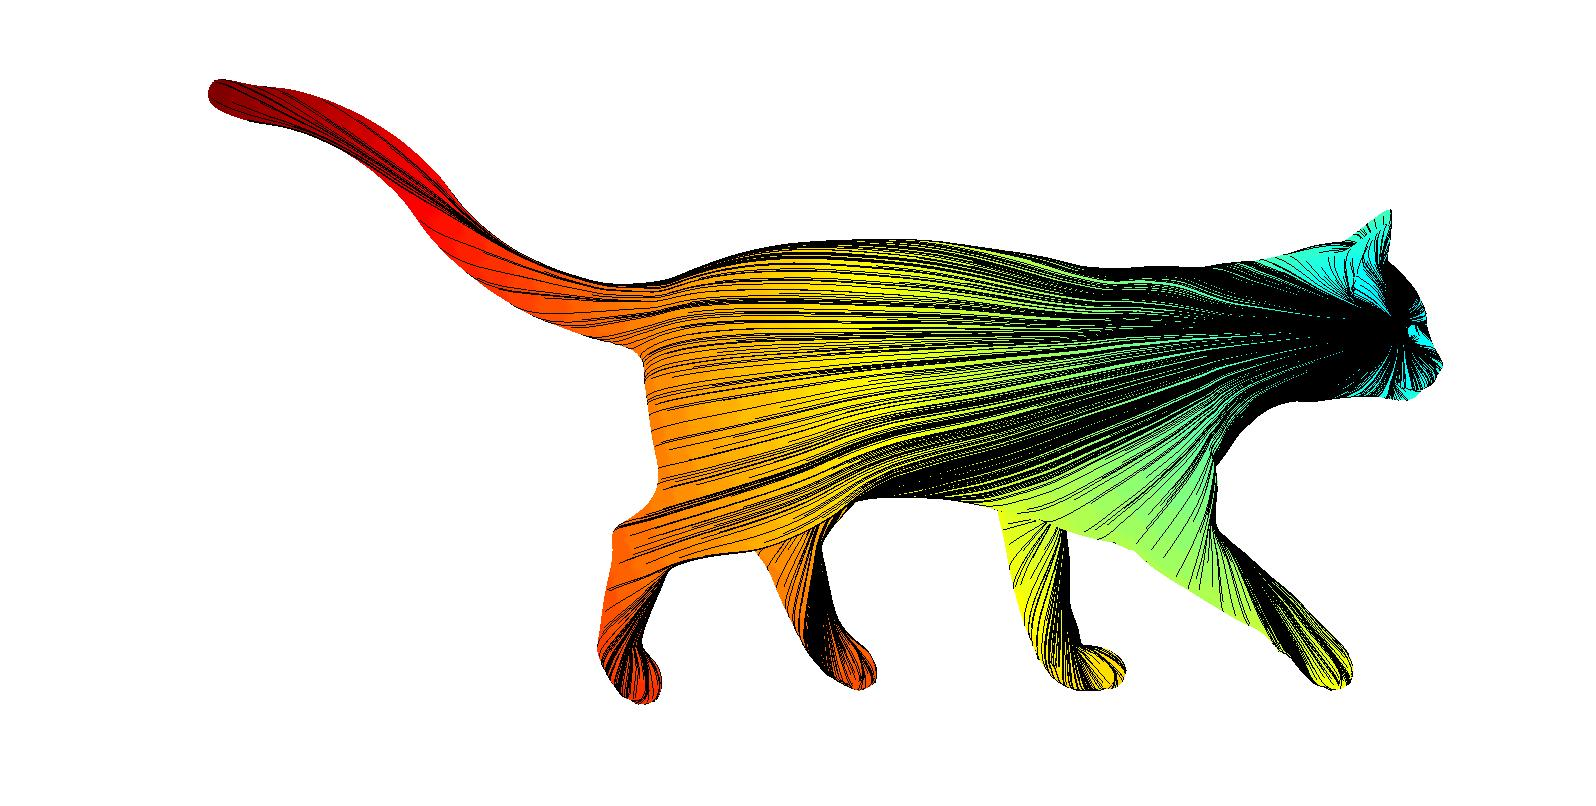
\includegraphics[width=0.8\textwidth]{t_pictures/cat_geodesic_paths}\\

		\note{note sure how much to tell here \ldots basic idea is to define a ``straight'' line between two points\\}
		\note{keywords: regular, parametrized curve, where the covariant derivative of its tangent vectors (projection of the (tangent) vectors derivative to the tangent plane)
			  is zero (called parallel vector field).\\}
		\note{intrinsic, since only dependent on covariant derivative, which can be expressed in Christoffel symbols, which are only dependent on the FFF\\}
		\note{for the existence of shortest geodesics, the surface has to be complete, otherwise there is the hole-example\\}
	\end{frame}

	\begin{frame}
		Discretisation to triangulated meshes:
		\begin{itemize}
			\item geodesics need to be straight lines within each face
			\item when crossing an edge, the geodesic has to correspond to a straight line if the adjacent faces are unfolded into a common plane
			\item distance information is propagated over the mesh in a Dijkstra-like manner by combining multiple geodesics into a single data structure called window
		\end{itemize}
		\includegraphics[width=\textwidth]{t_pictures/geodesics_new_windows} \\

		\note{alternative implementation: solving the eikonal equation using the fast marching method\\}
		\note{window parameters, propagation, intersection; resulting in windows that can be used to backtrack the geodesic distance\\}
		\note{special treatment of saddle/boundary vertices\\}
	\end{frame}

\subsection{Diffusion and Commute-Time Distance}
	\begin{frame}
		Diffusion Distance:\\
		\begin{itemize}
			\item measures the amount of heat transfered between two points after a certain time interval
			\item has a trade-off between local and global properties depending on a time parameter
		\end{itemize}
		%depends on time steps (2 pics) for local/global preference
		\pause
		Based on the Heat equation $\Delta_S u(x,t) = -\frac{\partial u(x,t)}{\partial t}$
		the formula for the diffusion distance can be obtained:
		$$ d_t^2(x,y) = \sum_{i=0}^{\infty} e^{-\lambda_i t} (\phi_i(x) - \phi_i(y))^2. $$

		\note{based on the standard heat kernel $k_t(x,y)$\\ average time to randomly walk x-y-x }
	\end{frame}

	\begin{frame}
		\begin{center}
			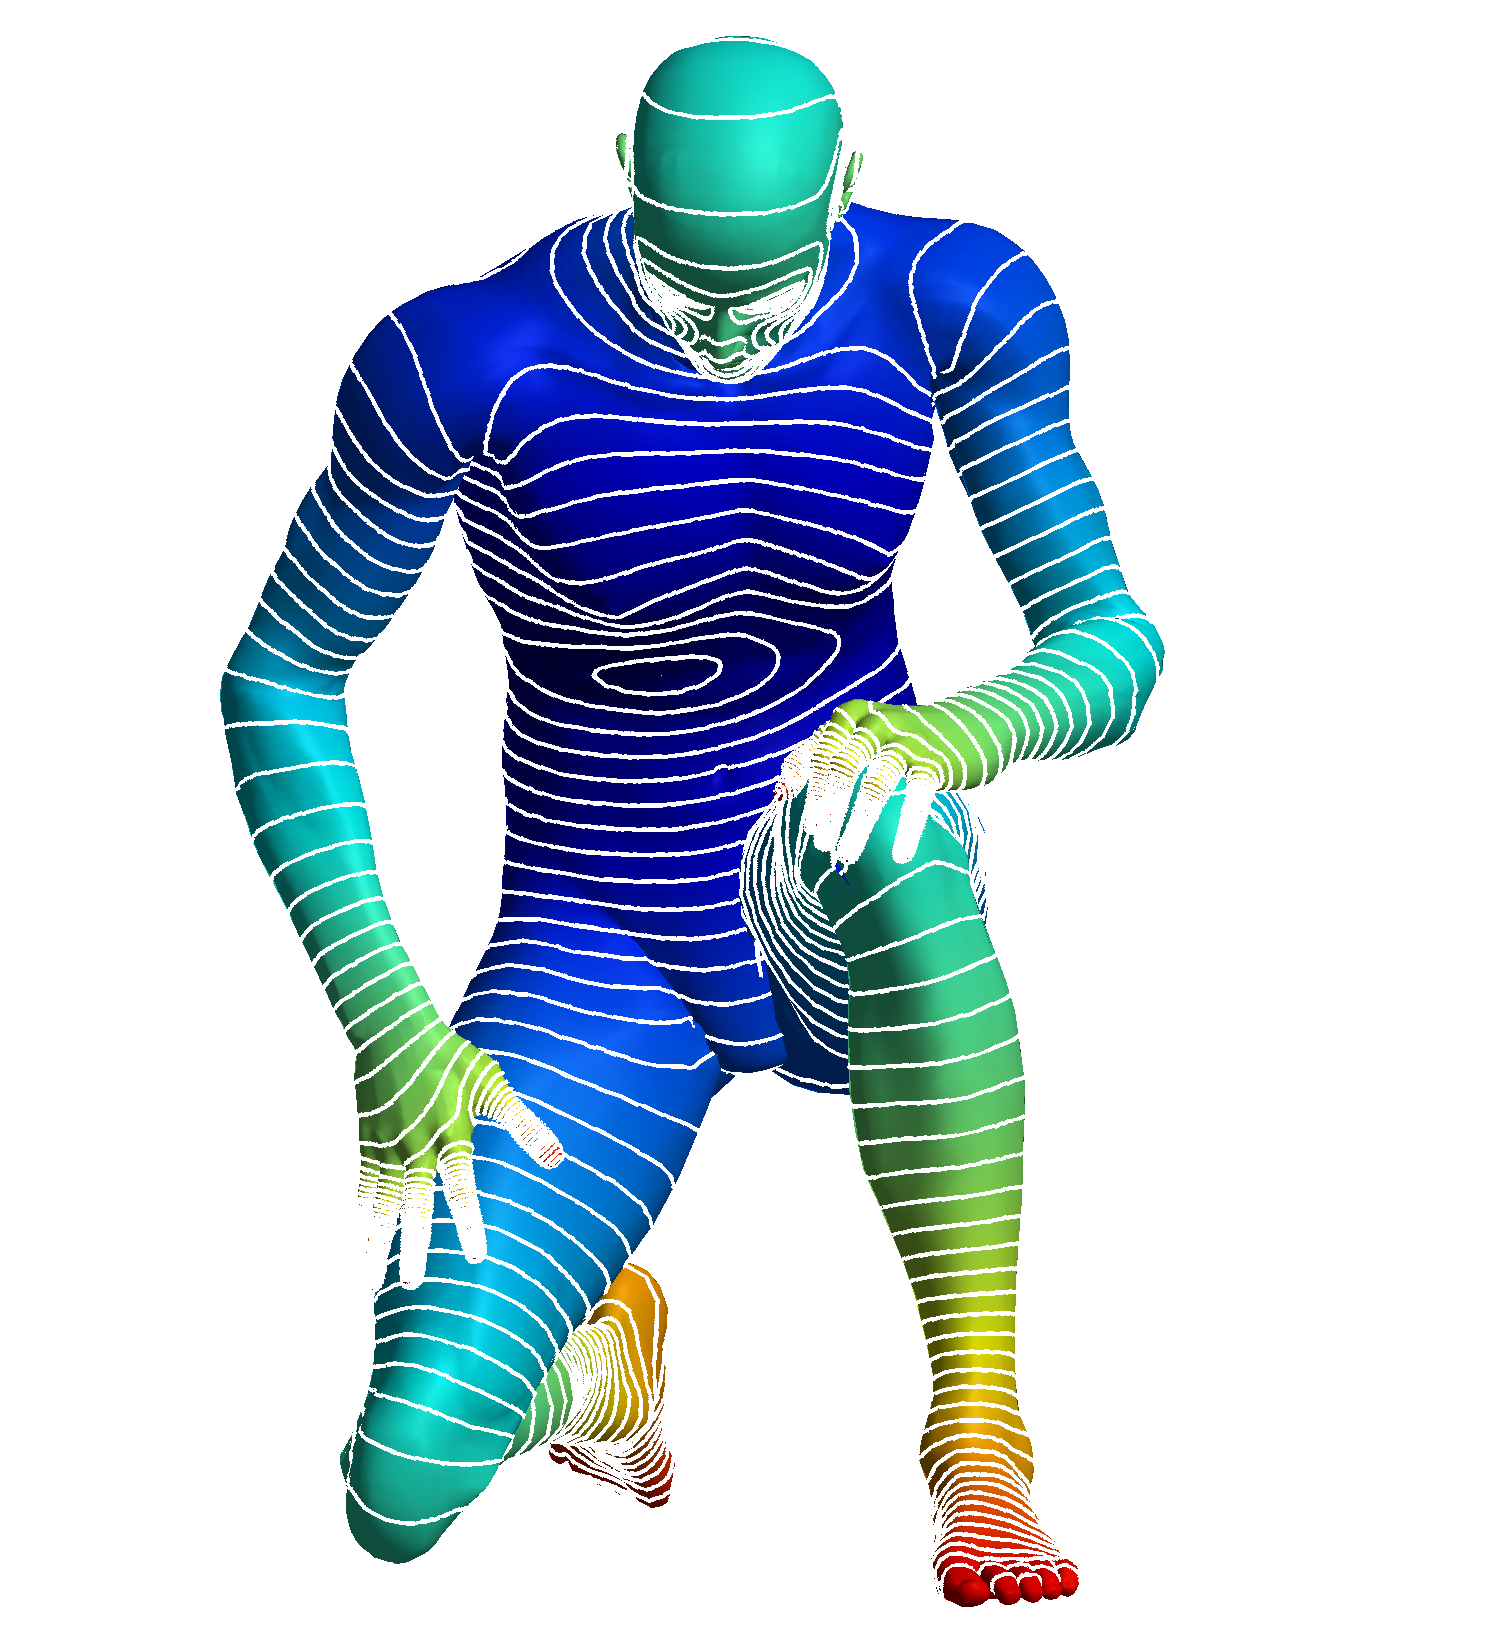
\includegraphics[width=0.4\textwidth]{diffusion_small_t.png}
			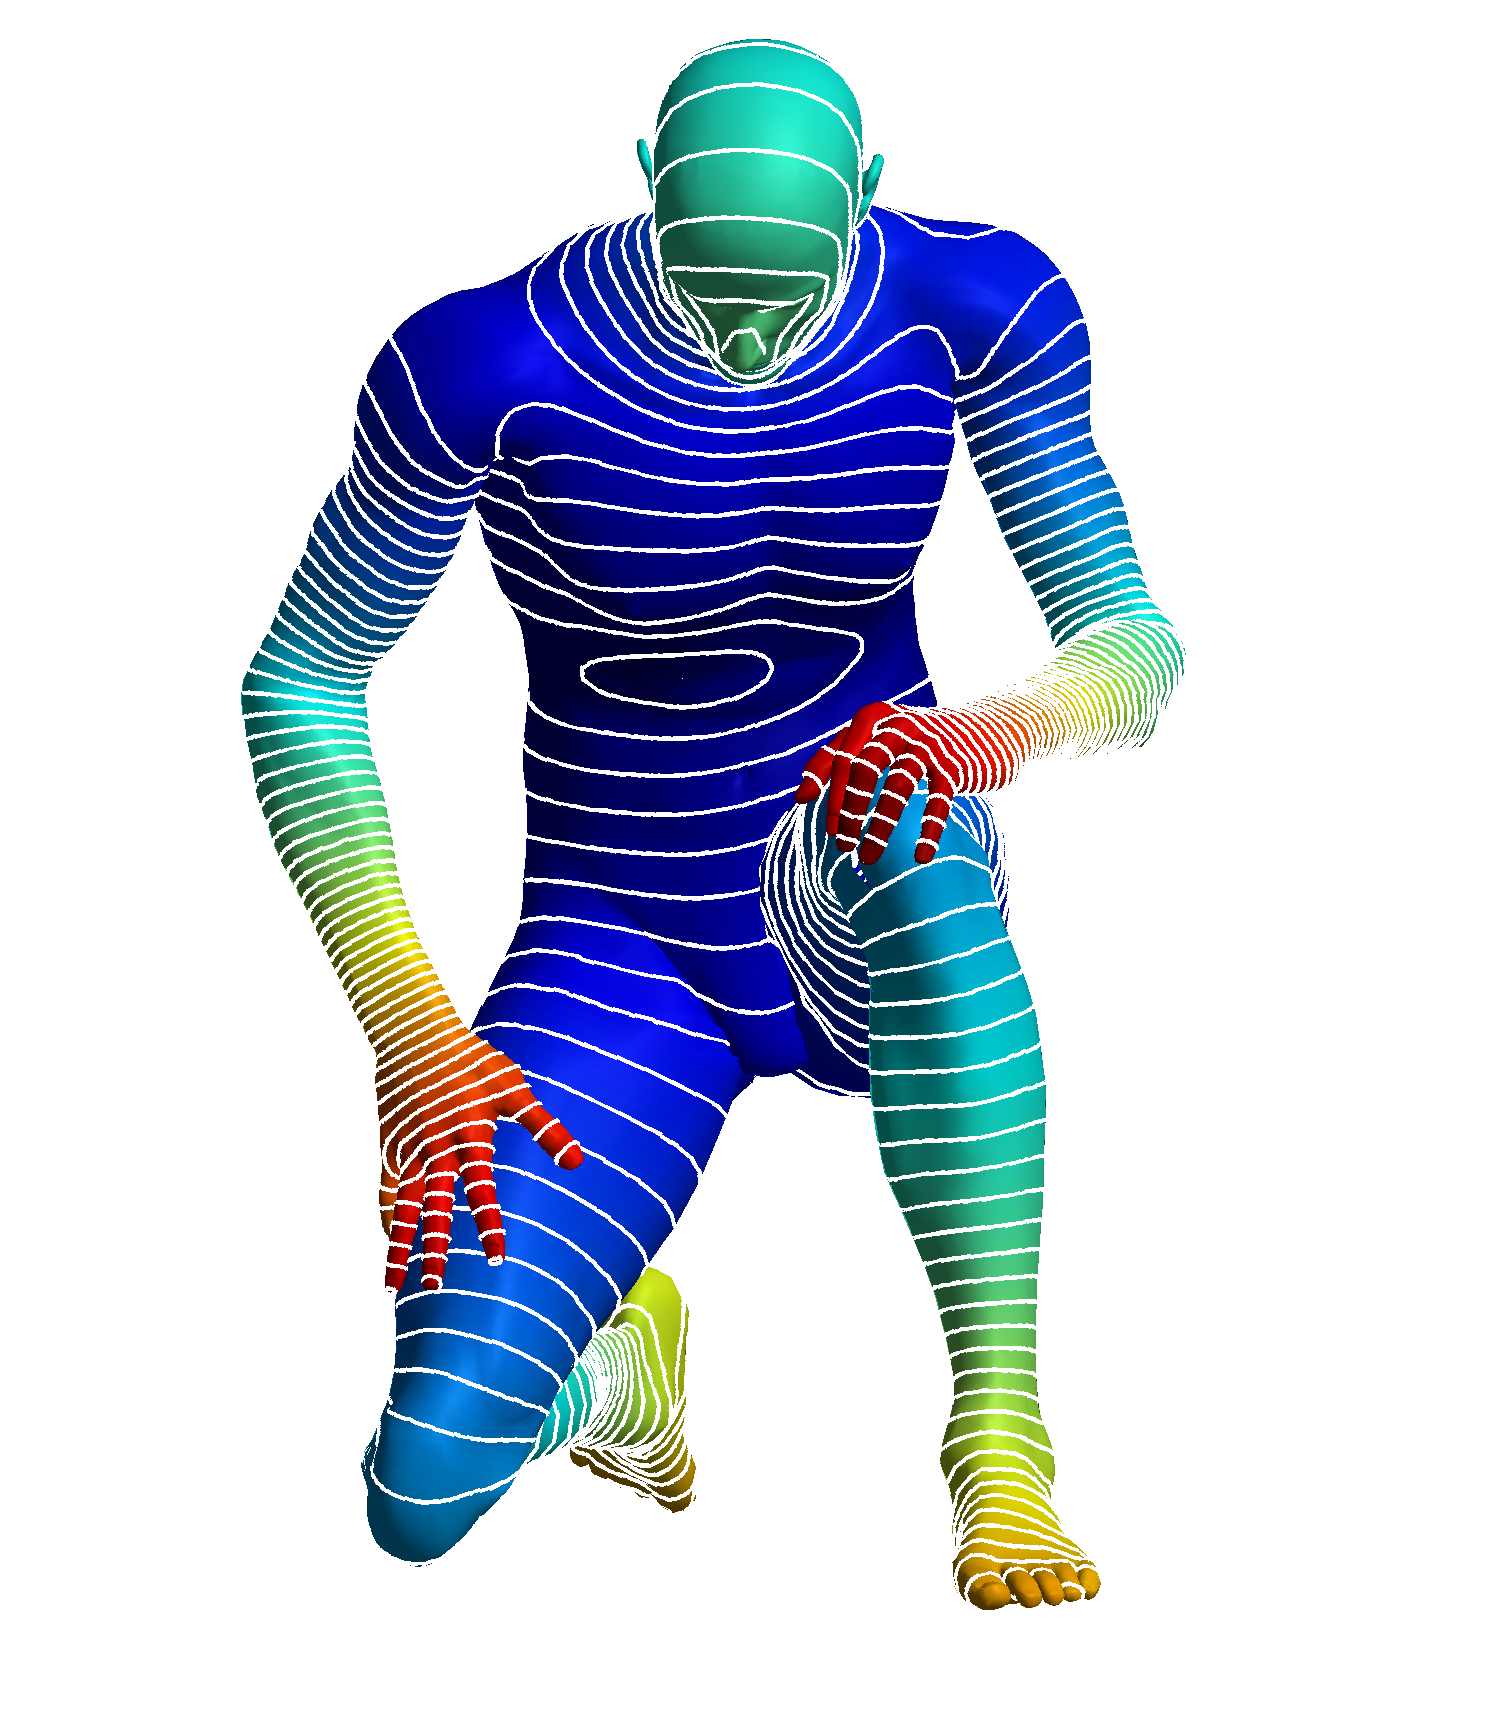
\includegraphics[width=0.4\textwidth]{diffusion_big_t.png}
		\end{center}
		
		\pause
		Commute-Time Distance:\\
		Integral of the Diffusion Distance over all time steps
		$$ d_C^2(x,y) = \sum_{i=0}^{\infty}  \frac{1}{-\lambda_i}(\phi_i(x) - \phi_i(y))^2. $$
		\note{
			\begin{itemize}
				\item Diffusion distance: to make it scale invariant, we rescaled $t \rightarrow t/\lambda_1$ (smallest eigenvalue not equal to zero)
				\item tries to combine local and global properties
				\item can be expressed using the heat kernel
					$k_t(x,y) = \sum_{i=0}^{\infty} e^{-\lambda_i t}\phi_i(x)\phi_i(y)$, leading to
					$d_t^2(x,y) = k_t(x,x) + k_t(y,y) - 2k_t(x,y)$
				\item Commute-time uses $k_C(x,y) = \sum_{i=0}^{\infty} \frac{1}{\lambda_i}\phi_i(x)\phi_i(y)$ as kernel (Green's function of the Laplacian)
				\item green's function = solution to inhomogenous differential equation; $LG(x,s) = \delta(x-s)$ $L$ is linear differential operator $L(x)$
			\end{itemize}
		}
	\end{frame}

\subsection{Biharmonic Distance}
	\begin{frame}
		Biharmonic Distance:\\
		\begin{itemize}
			\item newest metric, tries to combine the advantages of the other metrics
			\item based on the Green's function of the biharmonic differential equation
		\end{itemize}
		$$ d_B^2(x,y) = \sum_{i=0}^{\infty}  \frac{1}{\lambda_i^2}(\phi_i(x) - \phi_i(y))^2. $$

		\note{
			\begin{itemize}
				\item Lipman, Rustamov and Funkhouser (2010)
				\item found that 1/$\lambda$ decays to slow for their purposes, hence square it
				\item uses $k_B(x,y) = \sum_{i=0}^{\infty} \frac{1}{\lambda_i^2}\phi_i(x)\phi_i(y)$ as kernel
				\item good time to talk about truncating sums to approximate the distances/ that they are the same except for the factor (next slide helps)
			\end{itemize}
		}
	\end{frame}

	\begin{frame}
		$$ d_t^2(x,y) = \sum_{i=0}^{\infty} e^{-\lambda_i t} (\phi_i(x) - \phi_i(y))^2 $$
		$$ d_C^2(x,y) = \sum_{i=0}^{\infty}  \frac{1}{-\lambda_i}(\phi_i(x) - \phi_i(y))^2 $$
		$$ d_B^2(x,y) = \sum_{i=0}^{\infty}  \frac{1}{\lambda_i^2}(\phi_i(x) - \phi_i(y))^2 $$
	\end{frame}

\section{Testing and Implementation}
\subsection*{}
	\begin{frame}
		Testing goals:\\
		\begin{itemize}
			\item measure the computation speed
			\item visually compare the different metrics
			\item perform farthest point samplings based on different metrics
			\item analyse the relative error under isometries
		\end{itemize}

		\note{\begin{itemize}
			\item visual: different changes of the mesh (holes, localscale, noise, isometrie, topology changes)
			\item fps with euclidean (best anyway)
			\item error: usage of one to one correspondences
		\end{itemize}}
	\end{frame}

	\begin{frame}
		Challenges during programming:
		\begin{itemize}
			\item mesh errors for geodesic distance
			\item not enough isolines, so that some details were not visible first
			\item used the zero eigenvalue
			\item cut maximal values of commute-time for meshes with holes
		\end{itemize}

		\note{\begin{itemize}
			\item geodesic ``broke'' mostly for holes or down sampling
			\item used $\lambda_0$ for all computations, found the bug thanks to Dr.Rodola in the normalization of the diffusion distance
			\item commute-time: looked strange for a long time, until i fixed the next bug, leaving only strange behaviour of the metric as the cause
				%TODO picture of this?
		\end{itemize}}
	\end{frame}

\section{Results}
\subsection{Computation Speed}
	\begin{frame}
		\begin{table}[h]
			\begin{adjustbox}{max width=\textwidth}
			\begin{tabular}{@{}c*{6}{|r}|@{}}
				$|Vertices|$ &\begin{tabular}{@{}c@{}}Laplacian\\eigenfunctions\\/-values\end{tabular} & diffusion & \begin{tabular}{@{}c@{}}commute\\time\end{tabular}&
				biharmonic & \begin{tabular}{@{}c@{}}geodesic\\exact\end{tabular} & \begin{tabular}{@{}c@{}}geodesic\\Dijkstra\end{tabular}\\
				\hline
				1k  & 2.98   & 0.033 & 0.016 & 0.017 & 0.057  & 0.006 \\
				5k  & 12.46  & 0.122 & 0.064 & 0.070 & 0.481  & 0.014 \\
				10k & 30.35  & 0.283 & 0.157 & 0.169 & 1.449  & 0.036 \\
				20k & 65.08  & 0.487 & 0.268 & 0.288 & 3.632  & 0.063 \\
				50k & 206.58 & 1.193 & 0.655 & 0.705 & 12.123 & 0.149 \\
			\end{tabular}
			\end{adjustbox}
		\end{table}

		\note{using the first 200 eigenfunctions\\}
		\note{need to compute the (slow) Laplacian eigenfunctions first (but can be precomputed)\\}
		\note{only small differences for L-based metrics; geodesic much slower (for $V>5k$)\\}
		\note{geodesic: windows on each edge increase exponentially; dijkstra faster but worse\\}
	\end{frame}

\subsection{Visual comparison of the metrics}
	\note{interesting properties: locally isotropic, globally shape aware, insensitive to noise/topology, smooth\\}
	\note{from left to right: null-shape, isometry, noise, holes, local scale, topology\\}
	\note{geodesic: nice locally; but not globally shape aware (diagonal isolines on arms/cusps); not smooth at ridges\\}
	\note{diffusion: t=1/ t=0.1,0.05,0.01; first has good global properties, isolines perpendicular to central axis of arms/legs; close to source it gets closer to a circle the smaller t\\}
	\note{commute-time: scale invariant; but has local maxima (from small t), is not smooth; not stable with holes (removed max 60 of 50k)\\}
	\note{circular close, shape aware far away, best of all; only small changes at topology and local scale\\}
	\begin{frame}
		\hspace*{-0.5cm}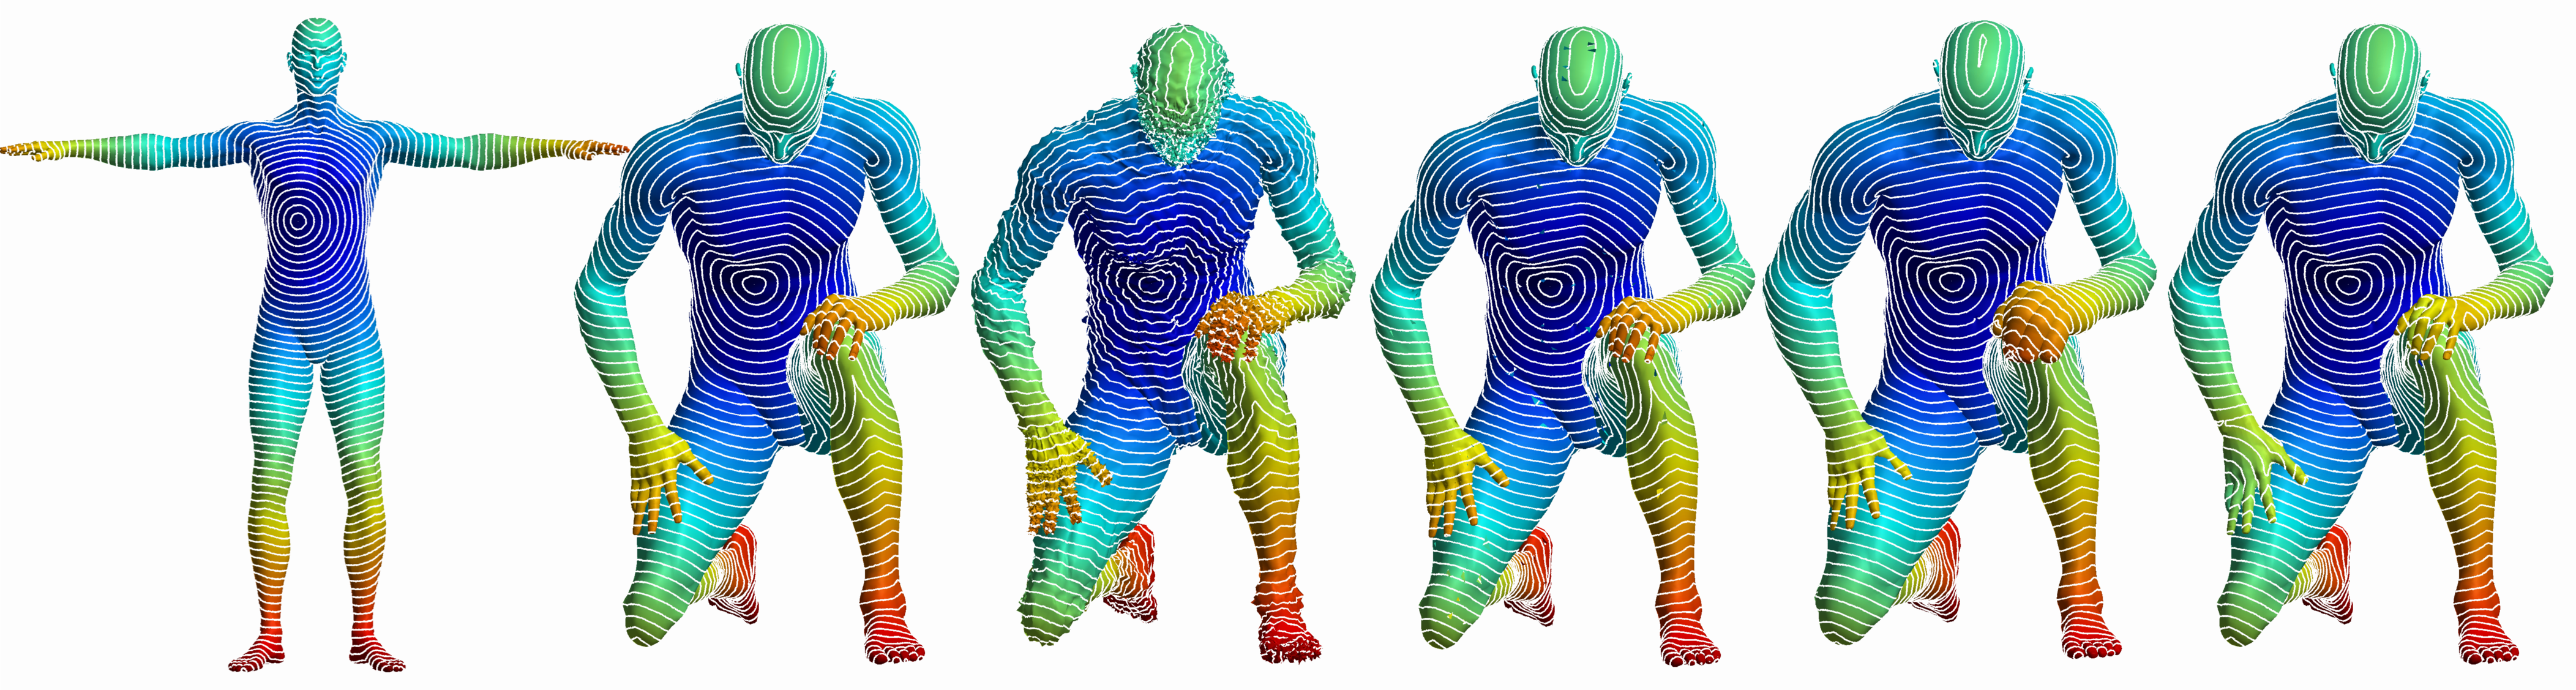
\includegraphics[width=1.1\textwidth]{results/geodesic_isolines.png}\\
		from left to right: null-shape, isometry, noise, holes, local scale, topology
	\end{frame}

	\begin{frame}
		\hspace*{-0.5cm}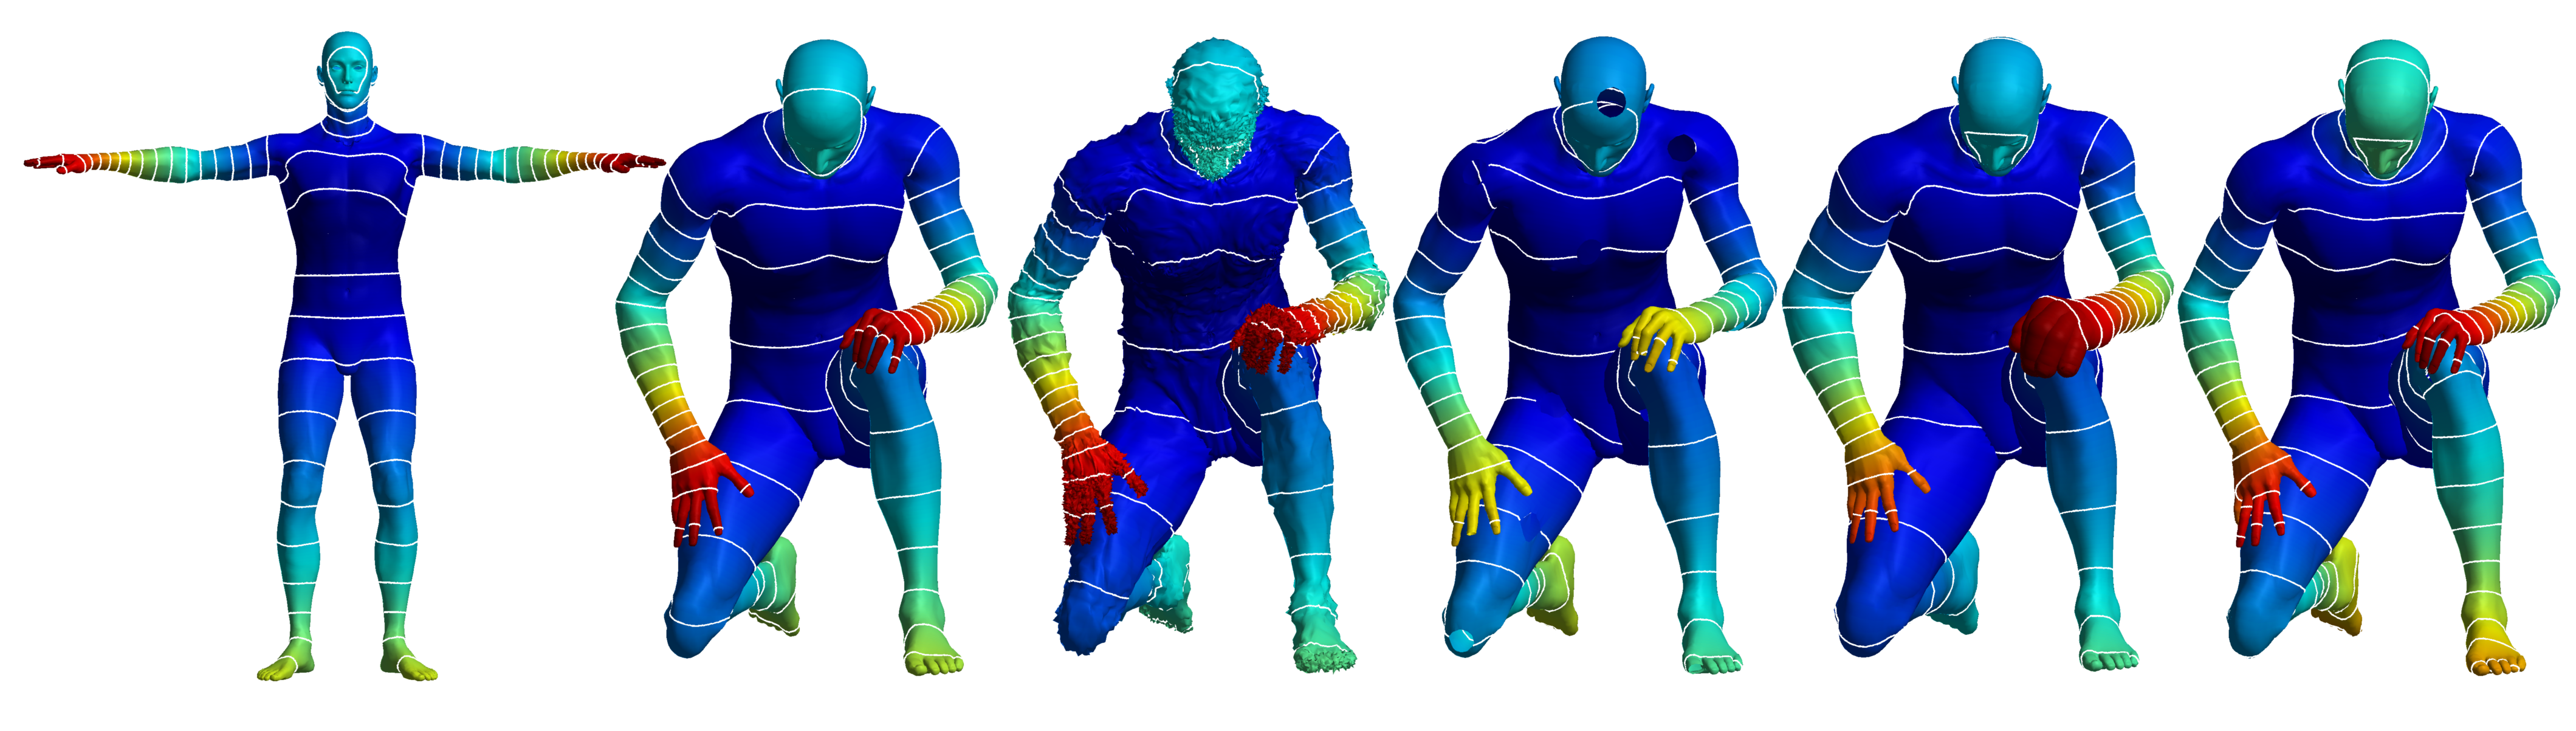
\includegraphics[width=1.1\textwidth]{results/diffusion_big_isolines.png}\\
		\pause
		\hspace*{-0.5cm}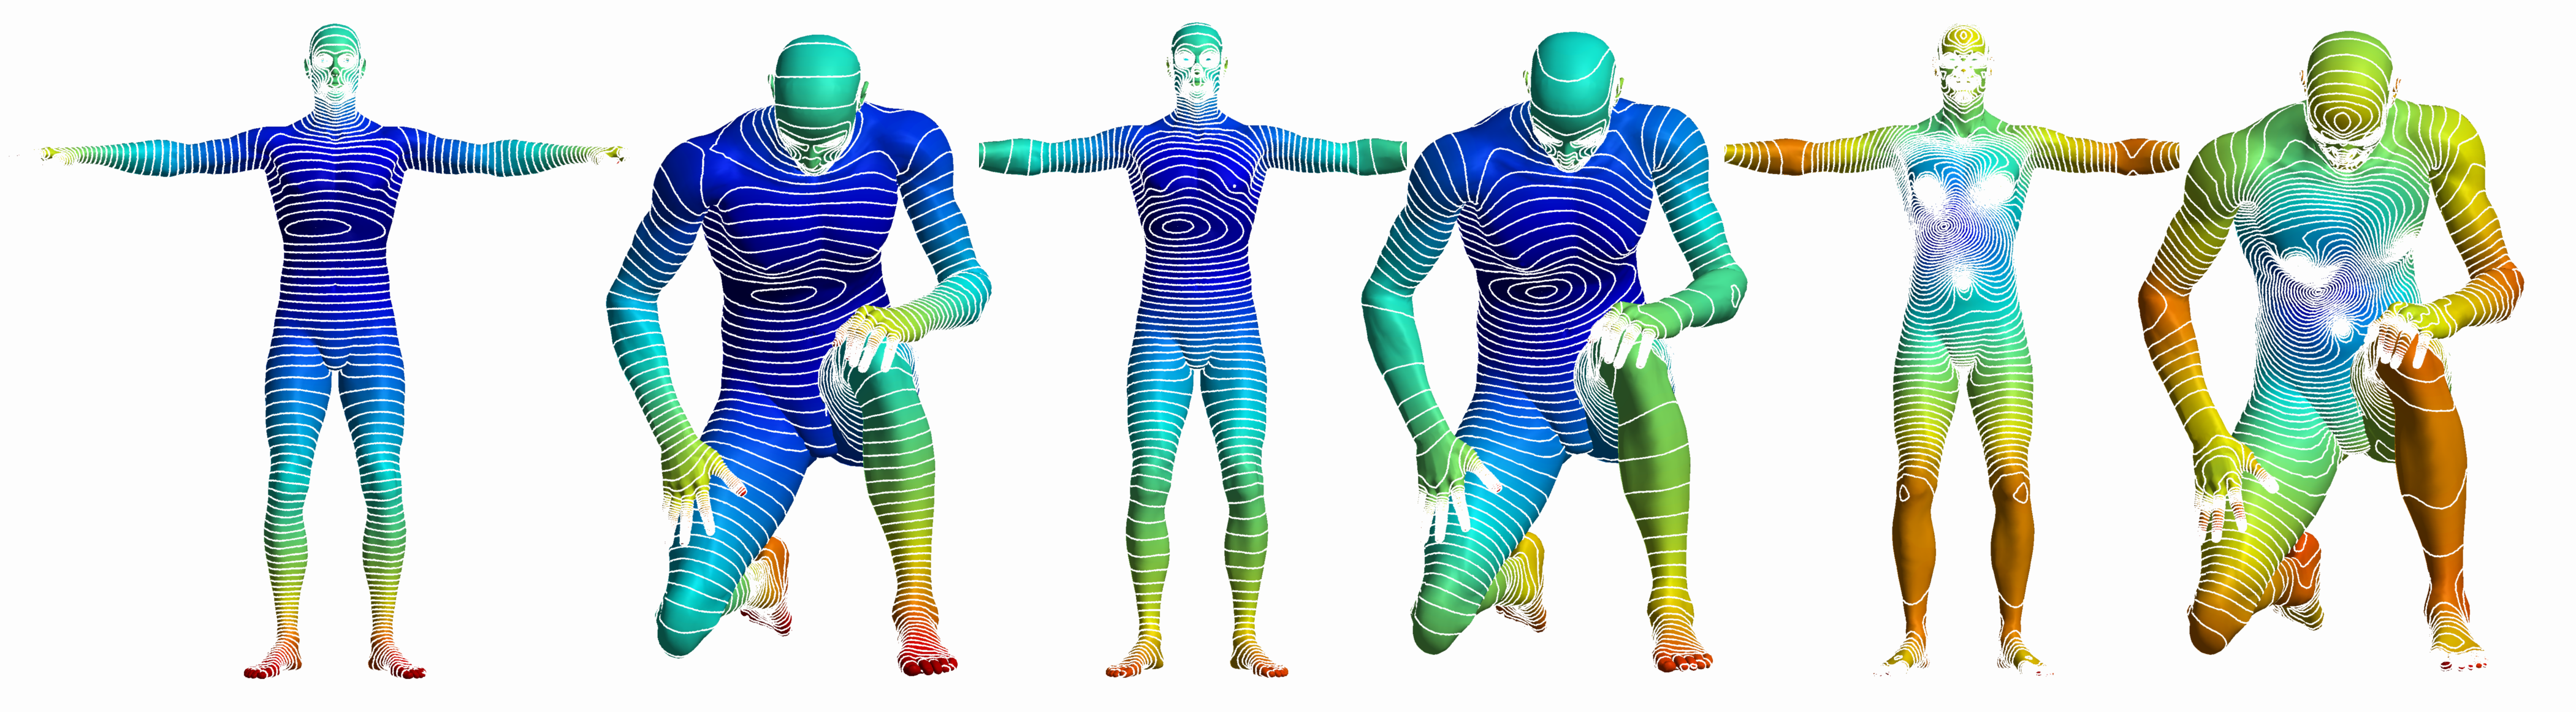
\includegraphics[width=1.1\textwidth]{results/diffusion_isolines_smaller_t.png}\\
		from left to right: null-shape, isometry, noise, holes, local scale, topology
	\end{frame}

	\begin{frame}
		\hspace*{-0.5cm}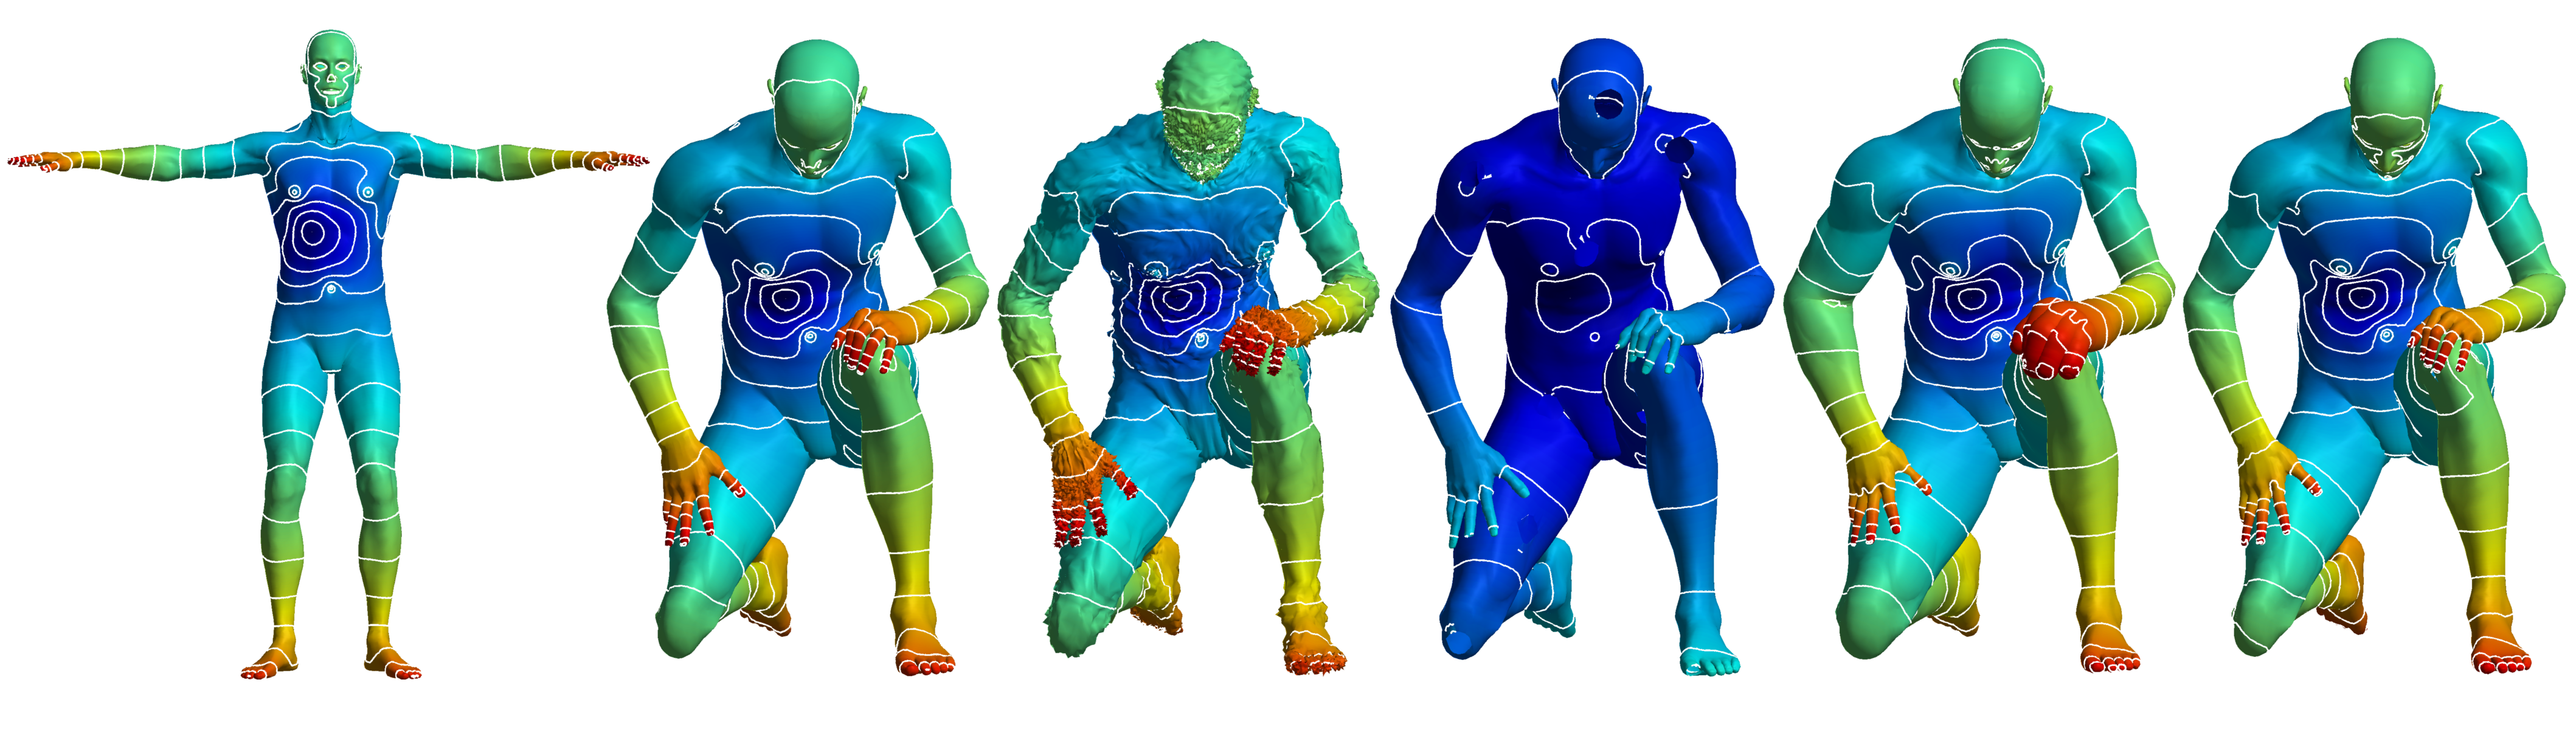
\includegraphics[width=1.1\textwidth]{results/commute_time_isolines.png}\\
		from left to right: null-shape, isometry, noise, holes, local scale, topology
	\end{frame}

	\begin{frame}
		\hspace*{-0.5cm}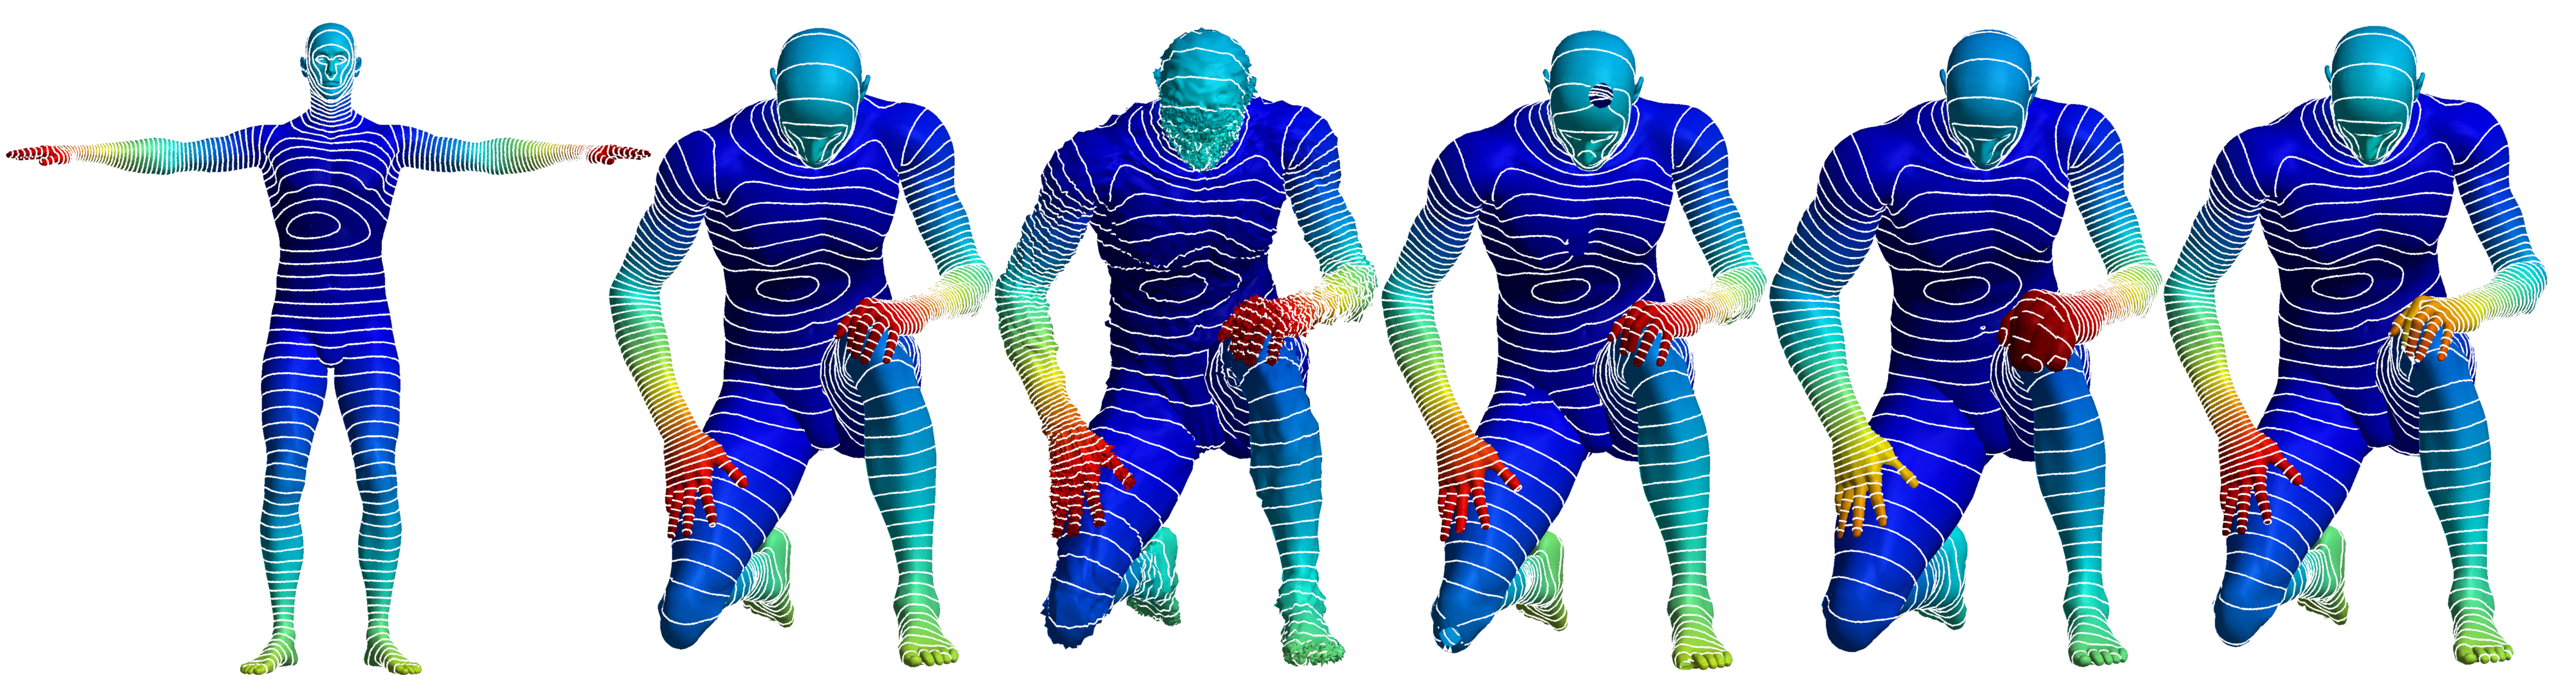
\includegraphics[width=1.1\textwidth]{results/biharmonic_isolines.png}\\
		from left to right: null-shape, isometry, noise, holes, local scale, topology
	\end{frame}

\subsection{Farthest point sampling}
	\begin{frame}
		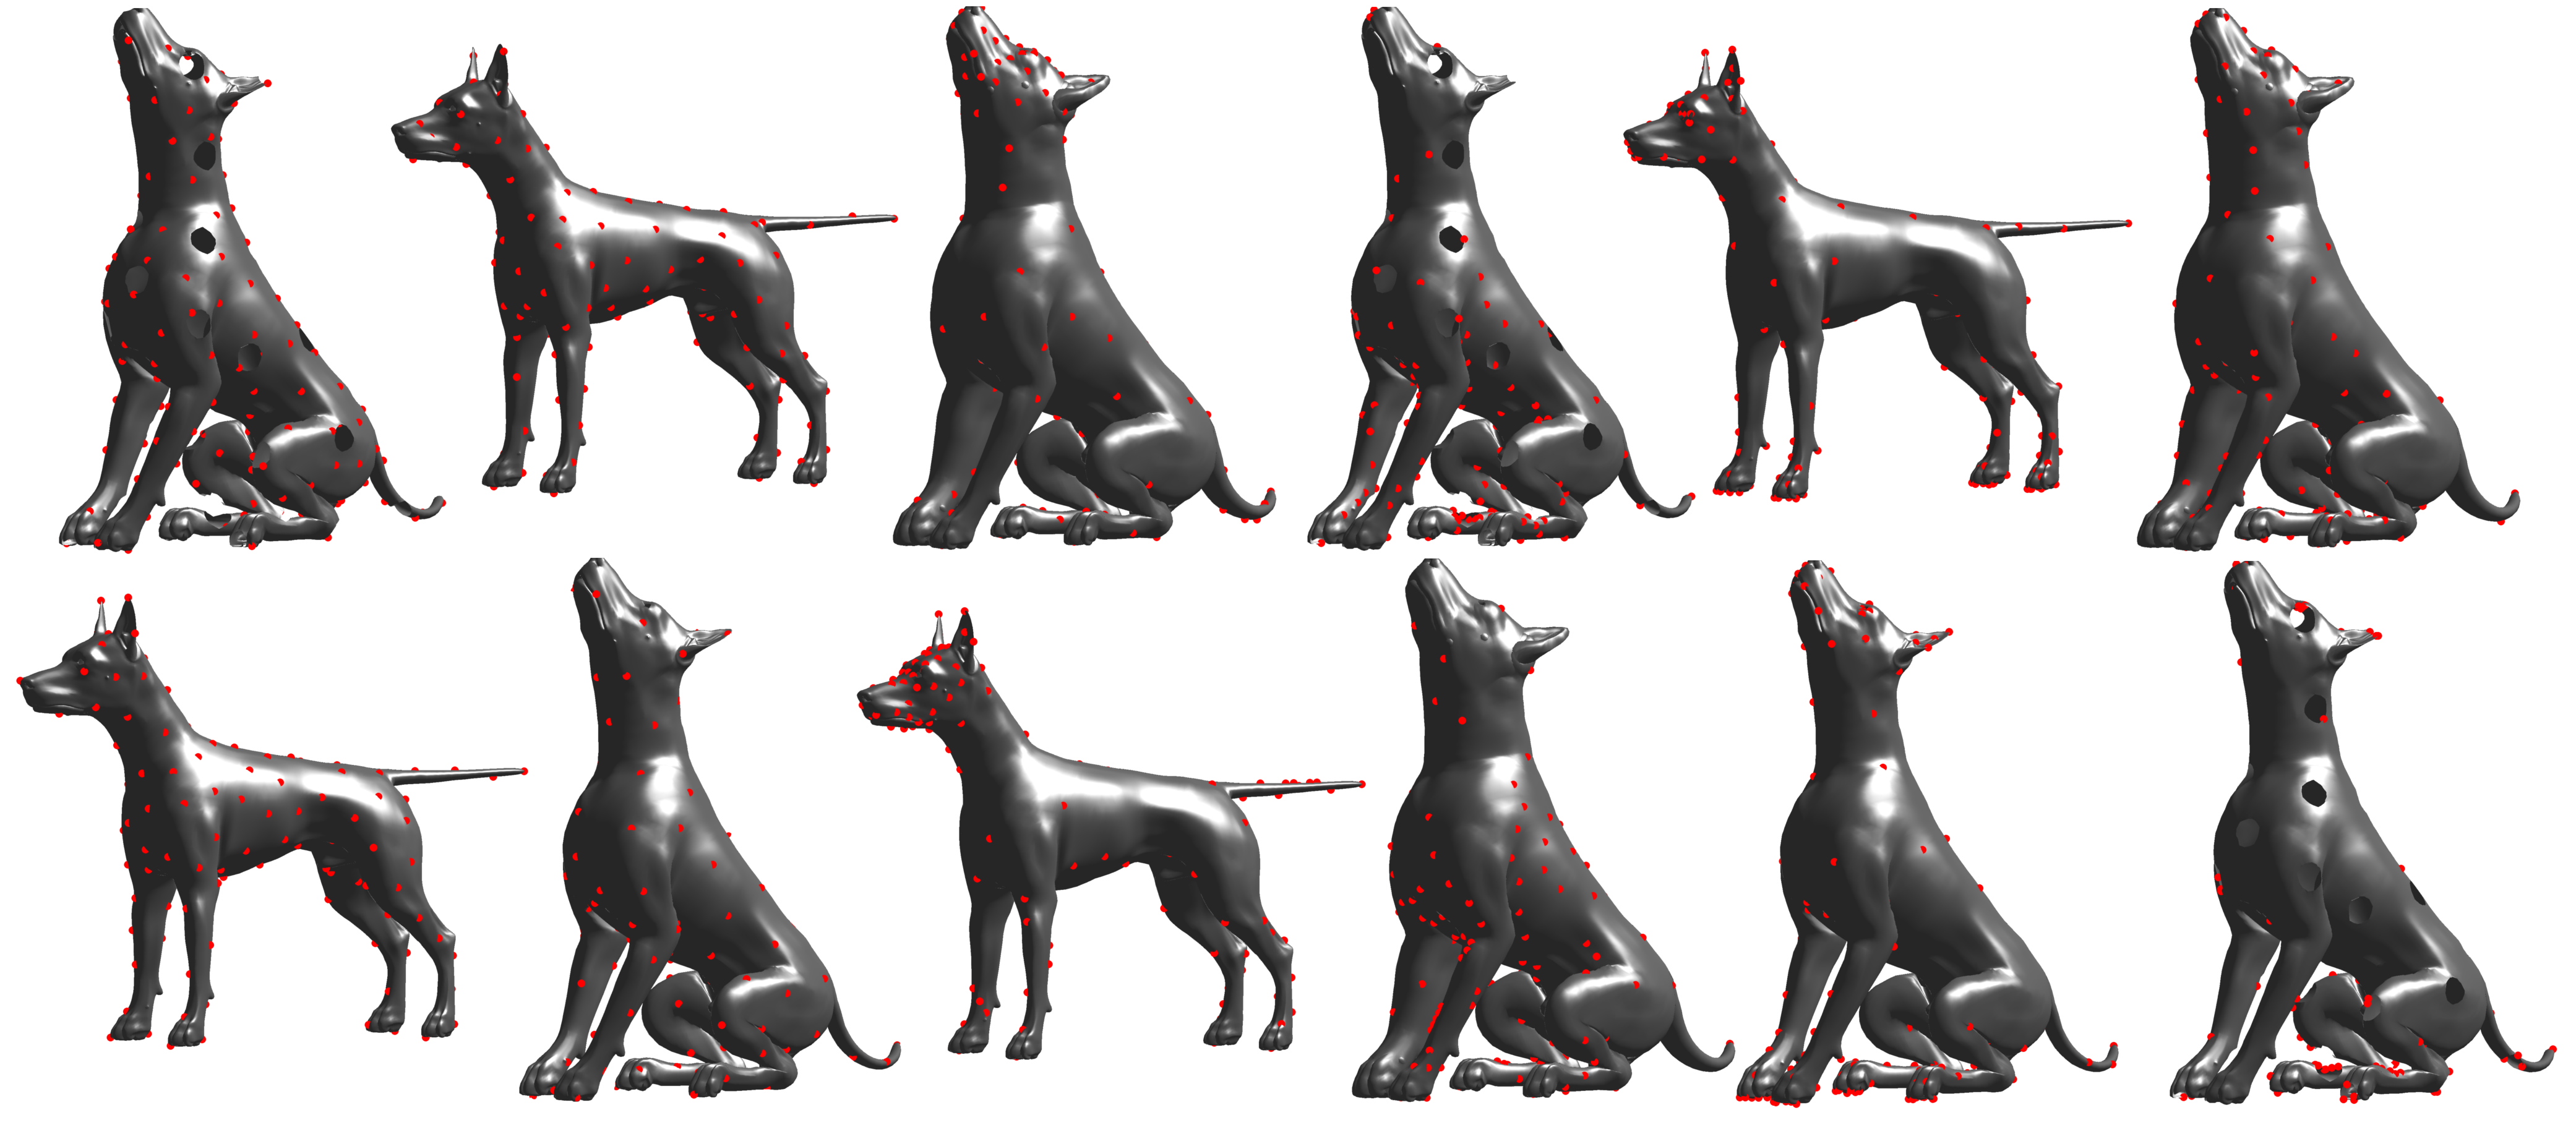
\includegraphics[width=\textwidth]{results/fps_end.png}\\
		from left to right: euclidean, geodesic, diffusion(2x), commute-time, biharmonic
		\note{from left to right: euclidean, geodesic, diffusion(2x), commute-time, biharmonic\\}
		\note{best results from euclidean; others either slow or cluster/leave blank spaces\\}
	\end{frame}

\subsection{Error analysis}
	\begin{frame}
		\begin{table}[h]
		\centering
		\begin{adjustbox}{max width=\textwidth}
			\begin{tabular}{@{}l*{8}{|r}|@{}}
				metric & isometry & \begin{tabular}{@{}c@{}}local\\scale\end{tabular} & scale & topology & noise & \begin{tabular}{@{}c@{}}shot\\noise\end{tabular} &
					\begin{tabular}{@{}c@{}}micro\\holes\end{tabular} & holes \\
				\hline
				geodesic		& .0232				& .0407				& .1580				& .0508				& .0218				& .0419				& .0417				& - \\
				diffusion t=0.1 & .0043				& .0310				& .0058				& .0408				& .0241				& .0044				& .0059				& .0434 \\
				diffusion t=1	& \underline{.0022} & .0320				& .0029				& .0223				& \underline{.0180} & \underline{.0018} & .0031				& .0528 \\
				commute-time	& .0034				& \underline{.0092} & .0037				& \underline{.0138} & .0309				& .0031				& .0035				& \underline{.0331} \\
				biharmonic		& .0049				& .0220				& \underline{.0016} & .0420				& .0625				& .0024				& \underline{.0017} & .0388 \\
			\end{tabular}
			\label{tab:mean}
		\end{adjustbox}
		\end{table}
		\note{maxerror was mostly won by the biharmonic distance 5/8\\}
		\note{no clear winner in mean error; geodesic $<$ small diffusion $<$ big diff/c-t $<$ biharmonic\\}
		\note{``hardest'' changes: noise, holes, topology\\}
	\end{frame}
%each for itself/together; watch, if my graphics are applicable or need to be made smaller

%conclusion: it was great i did that, because ...
	\begin{frame}
		Conclusions and further work:
		\begin{itemize}
			\item objective view on the properties of the metrics
			\item add the Earth mover's distance to the metrics
			\item use the FAUST dataset for testing
		\end{itemize}

		\note{biharmonic did best in errors/visual;\\ Earth mover's distance is a family of metrics\\}
	\end{frame}

\section*{}
	\begin{frame}
		\centering \large
		Thank you for your attention.\\
		Any Questions?
	\end{frame}

\section*{} %%appendix
\appendix
	\begin{frame}{Not enough isolines}
		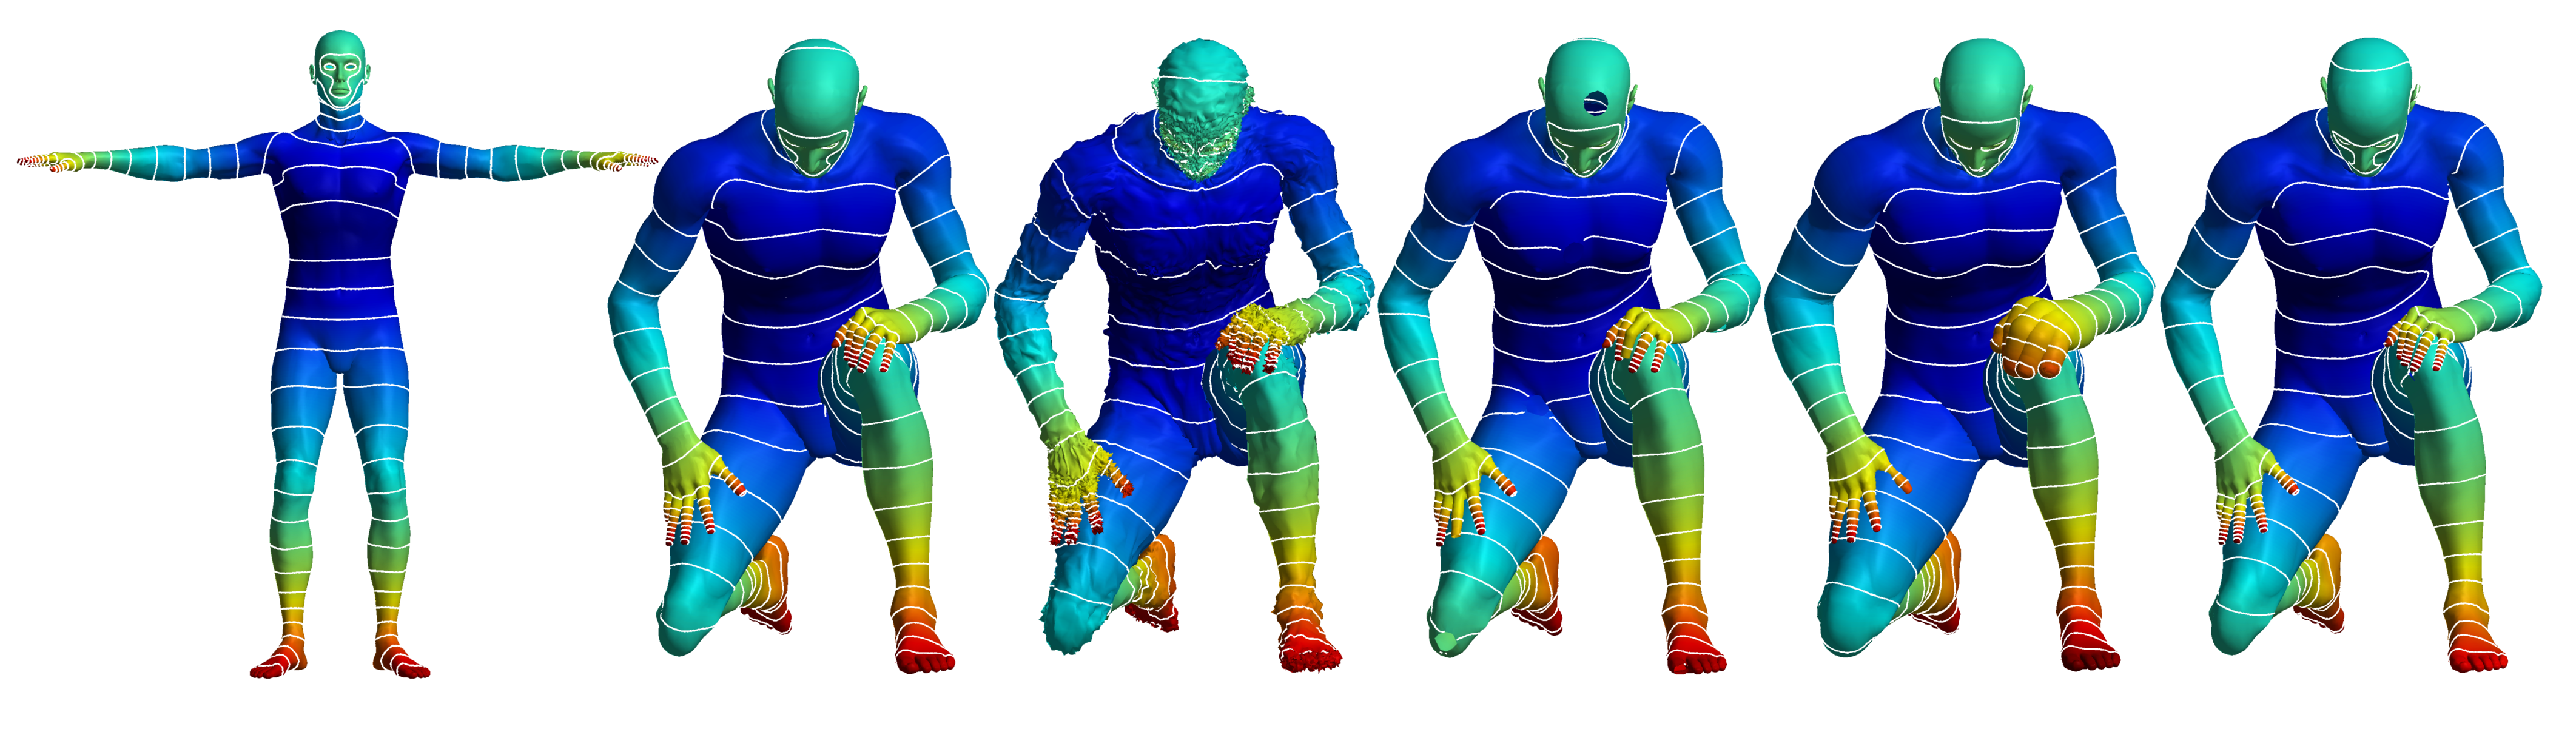
\includegraphics[width=0.9\textwidth]{results/diffusion_small_isolines.png}\\
	\end{frame}

\end{document}
